\section{Bureaucratic Processes}

Processes are designed to limit bad behavior or to allocate scarce resources

Does a process exist?



% https://graphthinking.blogspot.com/2015/07/notes-on-bureaucracy-and-social-network.html
Do participants know about existing processes?

\subsection{Processes involving two organizations}

When two independently-governed processes interact, there can be friction. Process friction, especially two uncoordinated organizations, results in either exceptions to the process or lying or change in process. 
Example: receipts from on process submitted for reimbursement to another process.
Submitting the receipt shifts the accountability and justification burden to the accepting bureaucrat.

% https://graphthinking.blogspot.com/2017/02/financial-motivation-in-bureaucracy.html

I have dental insurance. I visited the dentist December 2 and one of the procedures during a routine cleaning was ``bitewing x-rays." This procedure is covered by my insurance, so I was surprised when I received a bill for it from my dentist.

I called my dentist and they explained that the dental insurance had declined to pay for the procedure. I called the insurance company Jan 3 and they confirmed that the procedure was covered by my policy. 
Every time I call the insurance provider I have to provide my SSN, DoB, and Zip twice -- once to the automated system, a second time to the person I talk with. The insurance company apparently had made a mistake and said they would cover the cost of the procedure. I followed up with my dentist and explained the situation.

I called the dentist to see if they had received payment yet. They had not, so I called the dental insurance provider again Feb 6 and 8. Feb 8 the insurance company said they would process the payment within 7-10 business days. I called again Feb 20 and the claim hadn't been initiated within the insurance company. I spoke to the supervisor and she said she would personally visit the claims office within the insurance company.

From the perspective of the dentist, they are seeking money for the service they provided me.

From the perspective of the insurance company, delaying payment on a claim makes good financial sense -- the policy holder is likely to just pay the balance in order to avoid going to court with the dentist.

From my perspective, the question is whether chasing this issue makes financial sense. I think of my hourly rate as $40, so after an hour the charge of $38 would have been better to pay out of pocket. Effectively I'm devaluing my time. The emotional stress and thought-cycles expended are also relevant, though harder to quantify.


\href{https://en.wikipedia.org/wiki/Tragedy_of_the_commons}{Tragedy of the Commons} says that when there is a shared resource, someone will try to get away with behavior that is harmful to the organization.
Create processes for oversight/review/approval
Each process may be justifiable, but the aggregate is unreasonably burdensome


Deployment of processes and products need to account for 
normal users, Power users, malicious users, and edge cases



Processes with fewer people and fewer steps can be quicker and use fewer resources, but they are more fragile and less representative. Having more people involved helps with edge cases, but slows down the process. 

Any Nash equilibrium is constantly being upset by the change in conditions and change in people (who have varying motives).


Processes can be undocumented. Then oral folklore is the mechanism. 
    
Processes guardrails to prevent harm and keep stakeholders informed. 
    
Without oversight processes, \href{https://en.wikipedia.org/wiki/Tragedy_of_the_commons}{tragedy of commons} occurs and malicious actors dominate.
    


\begin{figure}
    \centering
    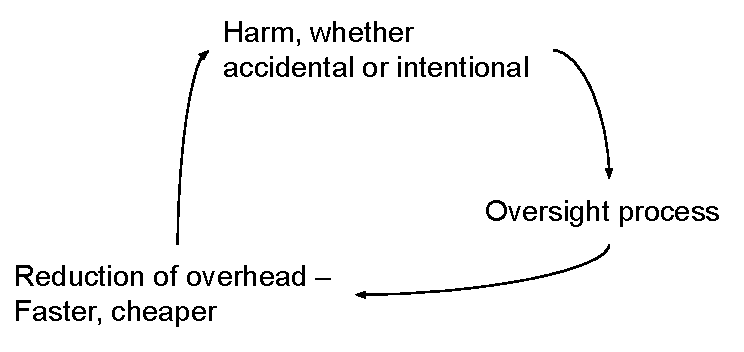
\includegraphics{images/process_loop_harm-oversight-improvement}
    \caption{loop: harm-oversight-improvement}
    \label{fig:harm-oversight-improvement}
\end{figure}


% https://graphthinking.blogspot.com/2021/04/laffer-curve-and-minimum-viable.html

\subsection{Processes as a tax on Productivity}

The Laffer curve is a claim in economics that there is a relation between government tax rates and the revenue from taxes collected. The relation, based on Rolle's theorem, says that between a tax rate of 0% and 100%, there must be some amount of tax that corresponds to the maximum of revenue. 

While the mathematical statement may be provable, the use in economics seems hand-wavy. In this post, I'll extend that hand-waviness to a different domain: bureaucratic processes in organizations. The relation to the Laffer curve is that bureaucratic processes a tax on productivity. 